% !TEX program = xelatex

\documentclass[10pt, compress,notheorems]{beamer}

\usetheme{m}

\usepackage{booktabs}
\usepackage[scale=2]{ccicons}
\usepackage{minted}
\usepackage{amsmath}
\usepackage{bm}
\usepackage{hyperref}
\usepackage{url}
\usepackage{graphicx}
\usepackage{multirow}
\usepackage{multicol}
\usepackage{amsfonts}
\usepackage{pgf,tikz}
\usepackage{tgpagella}
\usepackage{centernot}
\usepackage{caption}
\usepackage{xcolor}

\usepackage{graphicx}

\usepackage{xspace}
\newcommand{\themename}{\textbf{\textsc{metropolis}}\xspace}

\usepgfplotslibrary{dateplot}

\usemintedstyle{trac}

\title[Text Analysis]{Text Analysis}
\subtitle{}
\date{}
\author{
    \href{mailto:christopher.gandrud@city.ac.uk}{Christopher Gandrud}
}
\institute{SG1022, City University London}

\begin{document}

\maketitle

\frame{
    \frametitle{Aims}

    \begin{itemize}

        \item What is text analysis and why use it?

        \item Human coding

        \item Automated coding

        \item Pitfalls

    \end{itemize}

}

\section{Defining text analysis}

\frame{

    \begin{center}
        ``When we perform textual analysis on a text, we make an {\large{educated guess}} at some of the {\large{most likely interpretations}} that might be made of that text.'' {\small{(McKee 2003, 1)}}
    \end{center}
}

\frame{
    \frametitle{Define content analysis}

    \begin{center}
        ``{\large{Content Analysis}} is a research technique for making {\large{replicable and valid inferences}} from texts (or other meaningful matter [e.g. videos, audio]) to the {\large{contexts}} of their use.'' {\small{(Krippendorff 2013, 24)}}
    \end{center}
}

\frame{
    \frametitle{Replicable}

    \begin{center}
        \textcolor{gray}{``Content Analysis is a research technique for making {\large{replicable}} and valid inferences from texts (or other meaningful matter [e.g. videos, audio]) to the contexts of their use.''}
    \end{center}

    {\large{Replicable}}: different researchers, independent of each other should get the same results when applying the same technique.

    \vspace{0.5cm}

    E.g. independent researchers come to the understanding of the text using the same method.

    \vspace{0.5cm}

    Replicable results are more reliable.

}

\frame{
    \frametitle{Valid}

    \begin{center}
        \textcolor{gray}{``Content Analysis is a research technique for making replicable and {\large{valid}} inferences from texts (or other meaningful matter [e.g. videos, audio]) to the contexts of their use.''}
    \end{center}

    {\large{Valid}}: research is open to careful scrutiny and your claims can be upheld given independently available evidence.
}

\frame{
    \frametitle{Texts}

    \begin{center}
        \textcolor{gray}{``Content Analysis is a research technique for making replicable and valid inferences from {\large{texts}} (or other meaningful matter [e.g. videos, audio]) to the contexts of their use.''}
    \end{center}

    {\large{Texts}}: something that is produced by someone to have meaning for someone else.

    \vspace{0.5cm}

    E.g. newspaper articles, treaties, transcripts, tweets, maps, advertisements, press releases, movies, party manifestos.

    \vspace{0.5cm}

    In this course we focus exclusively on texts composed of words.

}

\frame{
    \frametitle{Texts in contexts}

    \begin{enumerate}

        \item<1-> Texts have no objective--reader-independent qualities. Meaning (data) arises from someone reading the text, often expecting other's understanding.

        \item<2-> Texts do not have single meanings.

        \item<3-> Meanings invoked by texts need not be shared.

        \item<4-> Contents refer to something other than themselves.

        \item<5-> Texts have meanings relative to particular contexts.

        \item<6-> Content analysts infer answers to particular research questions from their texts. Their inferences are merely more systematic, explicitly informed, and verifiable \ldots than what ordinary readers do.
    \end{enumerate}

}

\section{Why use text analysis?}

\frame{
    \frametitle{You}

    \begin{center}
        {\large{You \emph{use} and \emph{contribute} to text analysis}} {\large{every day.}}
    \end{center}
}

\frame{

    \begin{center}
        
\includegraphics[scale=0.45]{img/google_search_kanye.png}
    \end{center}
}

\frame{

    \begin{center}
        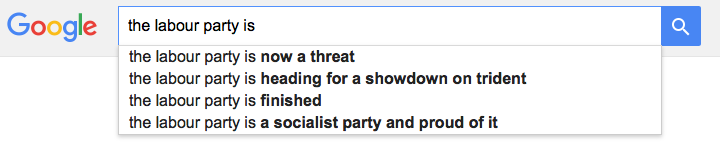
\includegraphics[scale=0.45]{img/google_search_labour.png}
    \end{center}

}

\frame{
    \frametitle{You}

    \begin{center}
        {\large{(Some of you) are building a data set that will be used for text analysis}} {\LARGE{right now}}.
    \end{center}

}

\frame{

    \begin{center}
        
\includegraphics[scale=0.45]{img/whats_app.png}
    \end{center}

{\tiny{Source: http://www.buzzfeed.com/shayanroy/blocking-you-now#.obE7eXDgAP}}

}

\frame{
    \frametitle{Social Science}

    \begin{center}
        People are creating {\large{increasingly more}} (machine accessible) texts.

        \vspace{1cm}

        {\large{Massive new source of data}} for social science analysis.
    \end{center}

}

\frame{
    \frametitle{Text analysis in social science (examples)}

    We may have research questions where we conducted a survey with an {\large{open-ended question}}.

    \vspace{1cm}

    We need some {\large{systematic way}} to {\large{understand}} these texts and {\large{make comparisons}} across survey respondents.

}

\frame{
    \frametitle{Text analysis in social science (examples)}

    We may have research questions where we want to interview a group of people that are hard to access, but who produce many texts.

    \vspace{1cm}

    For example, in an ideal world we may want to survey world leaders for their preferences to handling Syrian refugees. We may want to see how these preferences change over time.

    \vspace{1cm}

    World leaders don't given many interviews (especially not multiple interviews on the same topic), but they--often filtered through a press office--do create many texts.

}

\frame{
    \frametitle{German Chancellory Press Release Sept. 2015}


    \begin{center}
        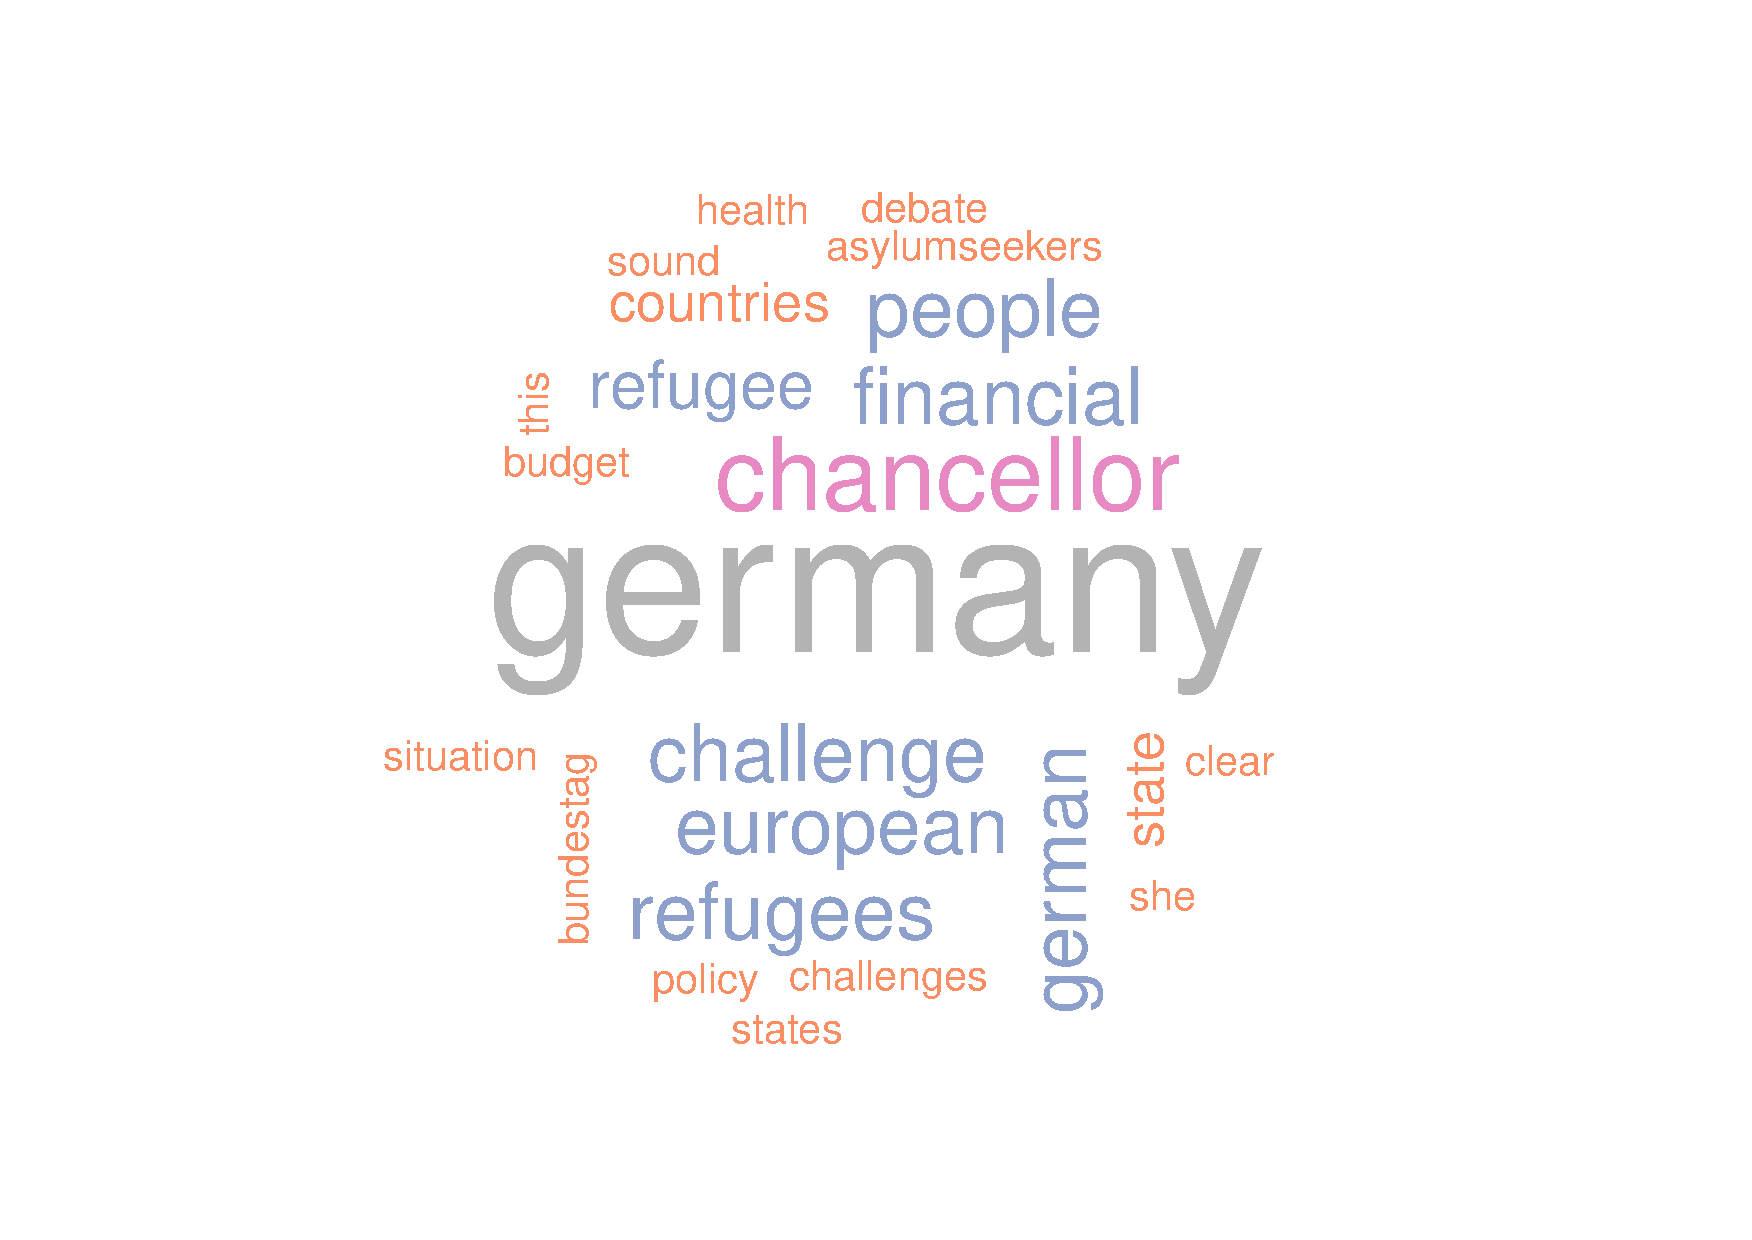
\includegraphics[scale=0.35]{img/sept_chancellor.pdf}
    \end{center}

}

\frame{
    \frametitle{Cologne New Years Eve Assults}

    \begin{center}
        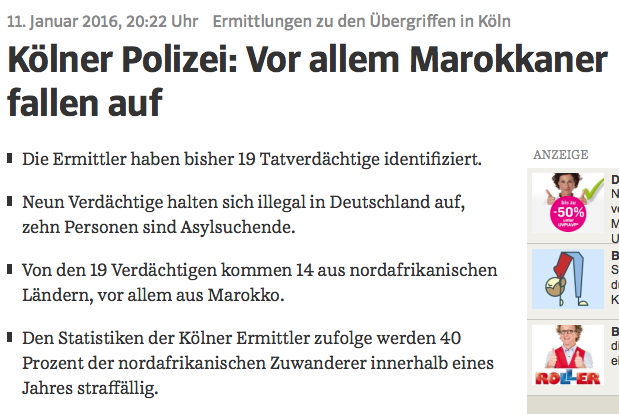
\includegraphics[scale=0.35]{img/sd_deutsche.png}
    \end{center}

    {\tiny{Source: http://www.sueddeutsche.de/panorama/ermittlungen-zu-den-uebergriffen-in-koeln-vor-allem-marokkaner-fallen-auf-1.2814336}}

}

\frame{
    \frametitle{Cologne New Years Eve Assults}

    \begin{center}
        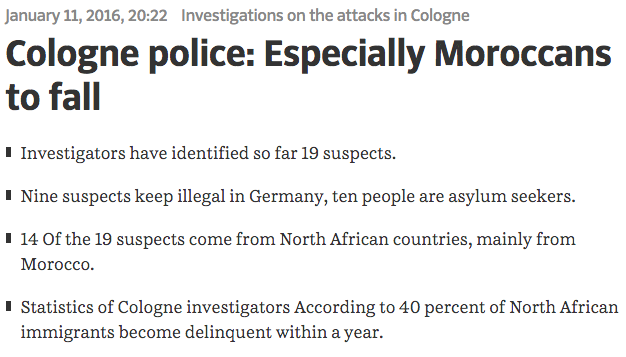
\includegraphics[scale=0.35]{img/sd_english.png}
    \end{center}

    {\tiny{Source: http://www.sueddeutsche.de/panorama/ermittlungen-zu-den-uebergriffen-in-koeln-vor-allem-marokkaner-fallen-auf-1.2814336 via Google Translate}}

}

\frame{
    \frametitle{German Chancellory Press Release January 2015}


    \begin{center}
        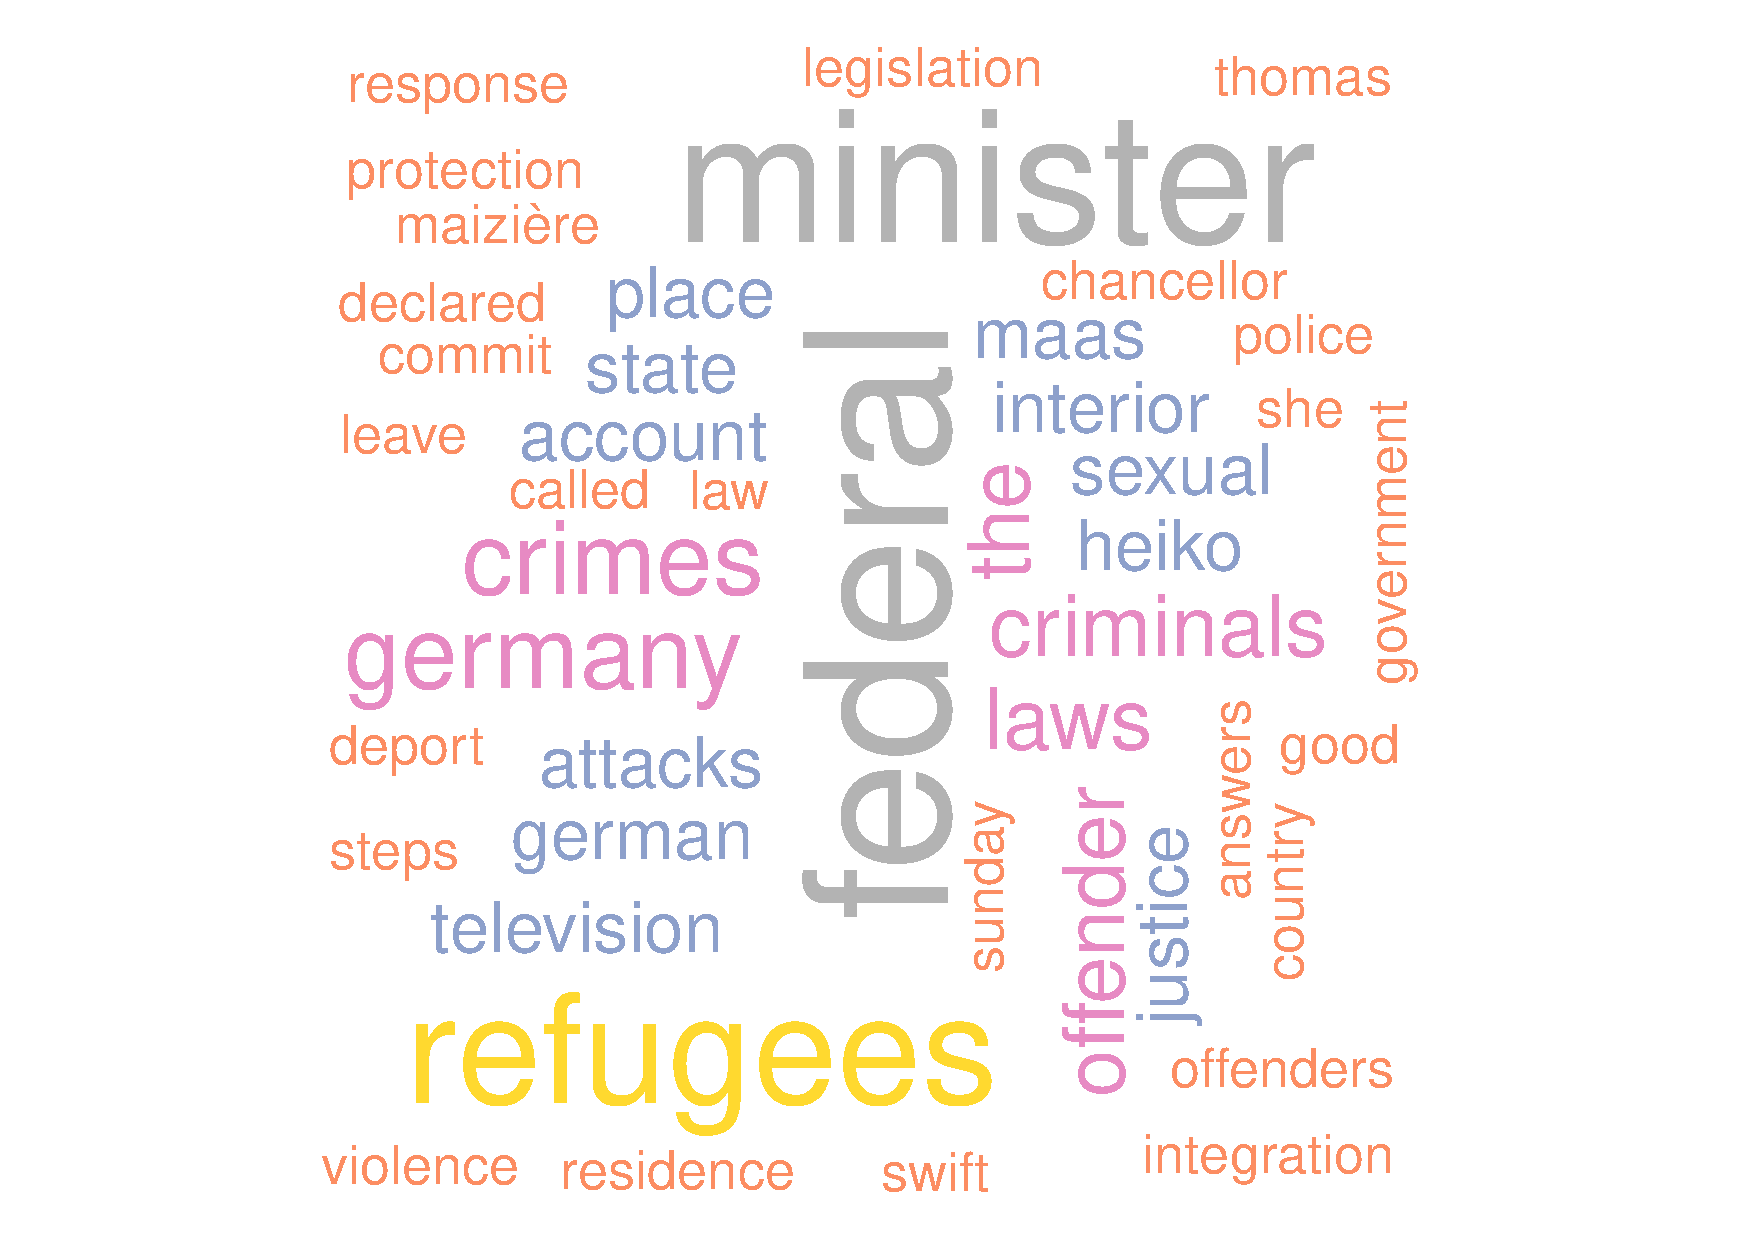
\includegraphics[scale=0.35]{img/jan_chancellor.pdf}
    \end{center}

}

\frame{
    \frametitle{Text analysis in social science (examples)}

    We may have research questions about units that are not able to be surveyed, but which produce texts.

    \vspace{1cm}

    E.g. International organisations, political parties, neighbourhood groups.
}

\frame{
    \frametitle{Comparative Party Manifestos Project}

    Left-Right Position of UK Parties Based on their Party Manifestos

    \begin{center}
        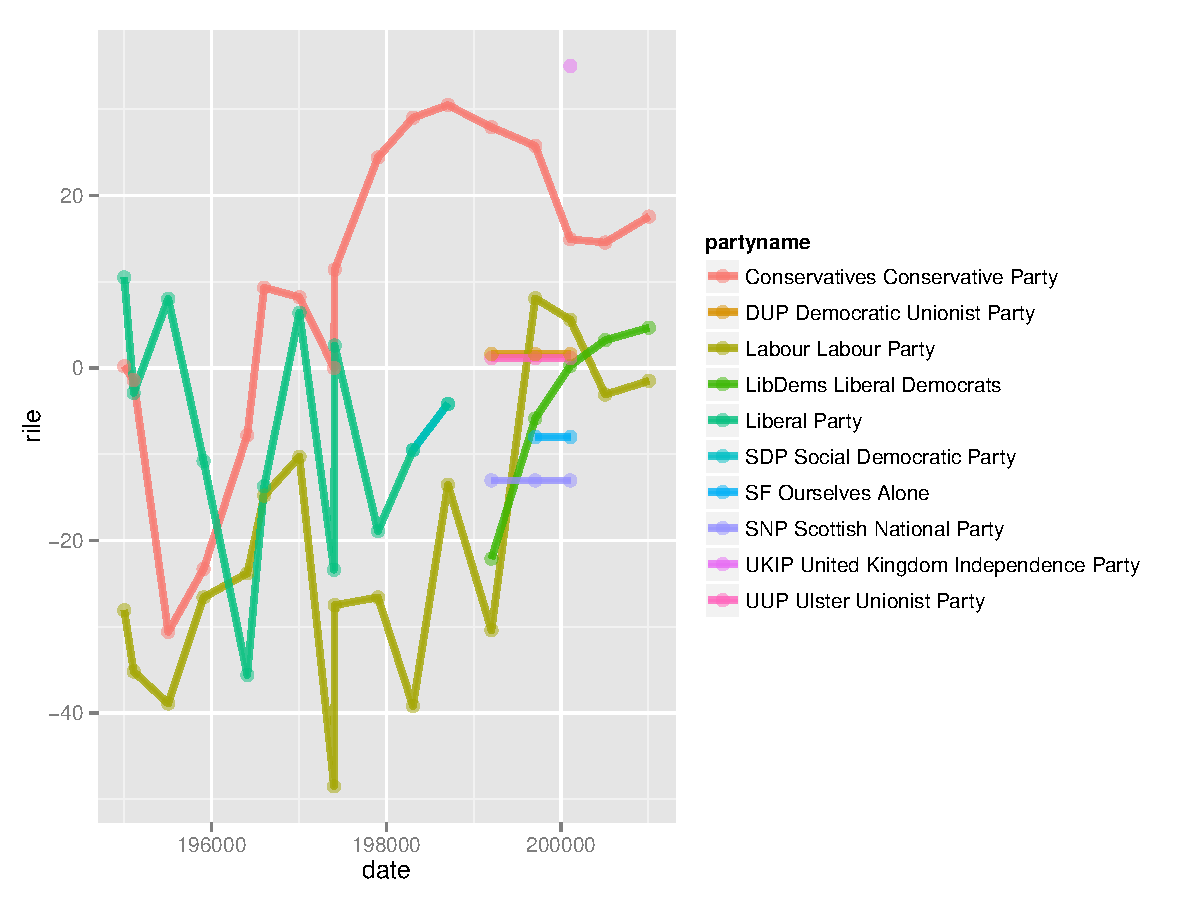
\includegraphics[scale=0.4]{img/uk_party_lr.pdf}
    \end{center}

    {\tiny{Source: https://visuals.manifesto-project.wzb.eu/mpdb-shiny/cmp\_dashboard/}}

}

\frame{
    \frametitle{Text analysis in social science (examples)}

    We may have research questions about {\large{how actors communicate}} to achieve goals.

    \vspace{1cm}

    For example, what topics do monetary policy bureaucrats talk about more when there is a financial crisis?

}

\frame{
    \frametitle{Topics of US Federal Reserve Governor Speeches}


    \begin{center}
        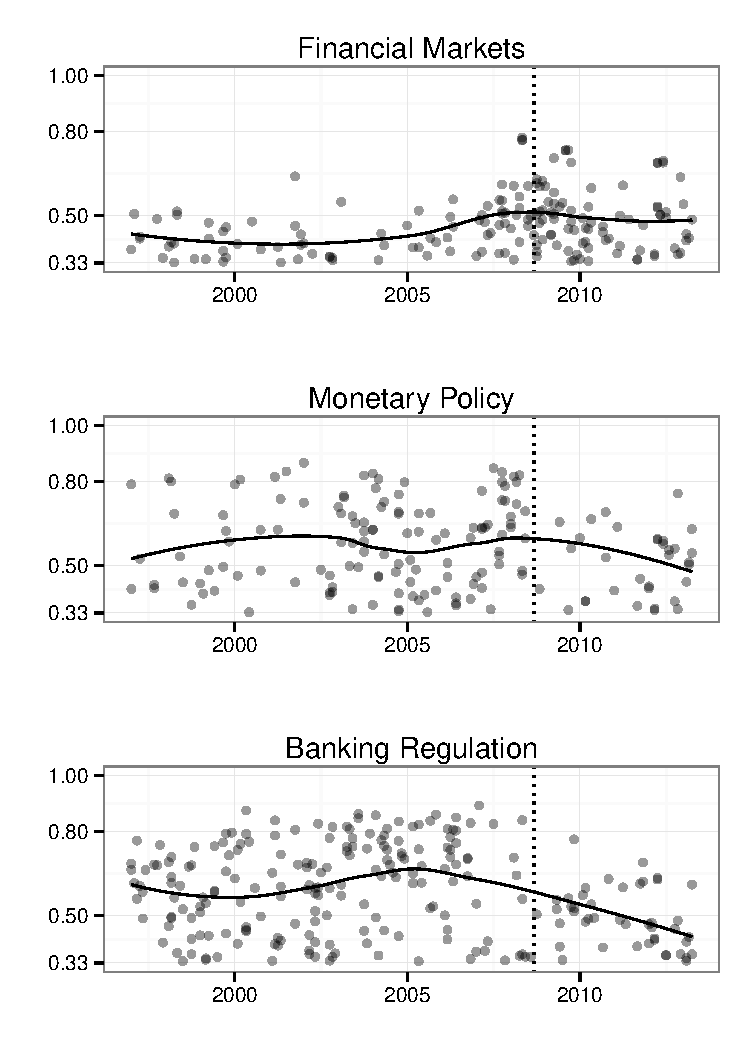
\includegraphics[scale=0.35]{img/TopicBasic.pdf}
    \end{center}

    {\tiny{Source: Young and Gandrud (2016)}}

}

\frame{
    \frametitle{Text analysis in social science (examples)}

    We may have research questions about widely held beliefs across time, where a survey would be {\large{too costly}} to run.

    \vspace{1cm}

    For example, if we wanted to study monthly perceptions of financial market stress across 180 countries.

}

\frame{
    \frametitle{Real-Time Perceptions of Financial Market Stress}


    \begin{center}
        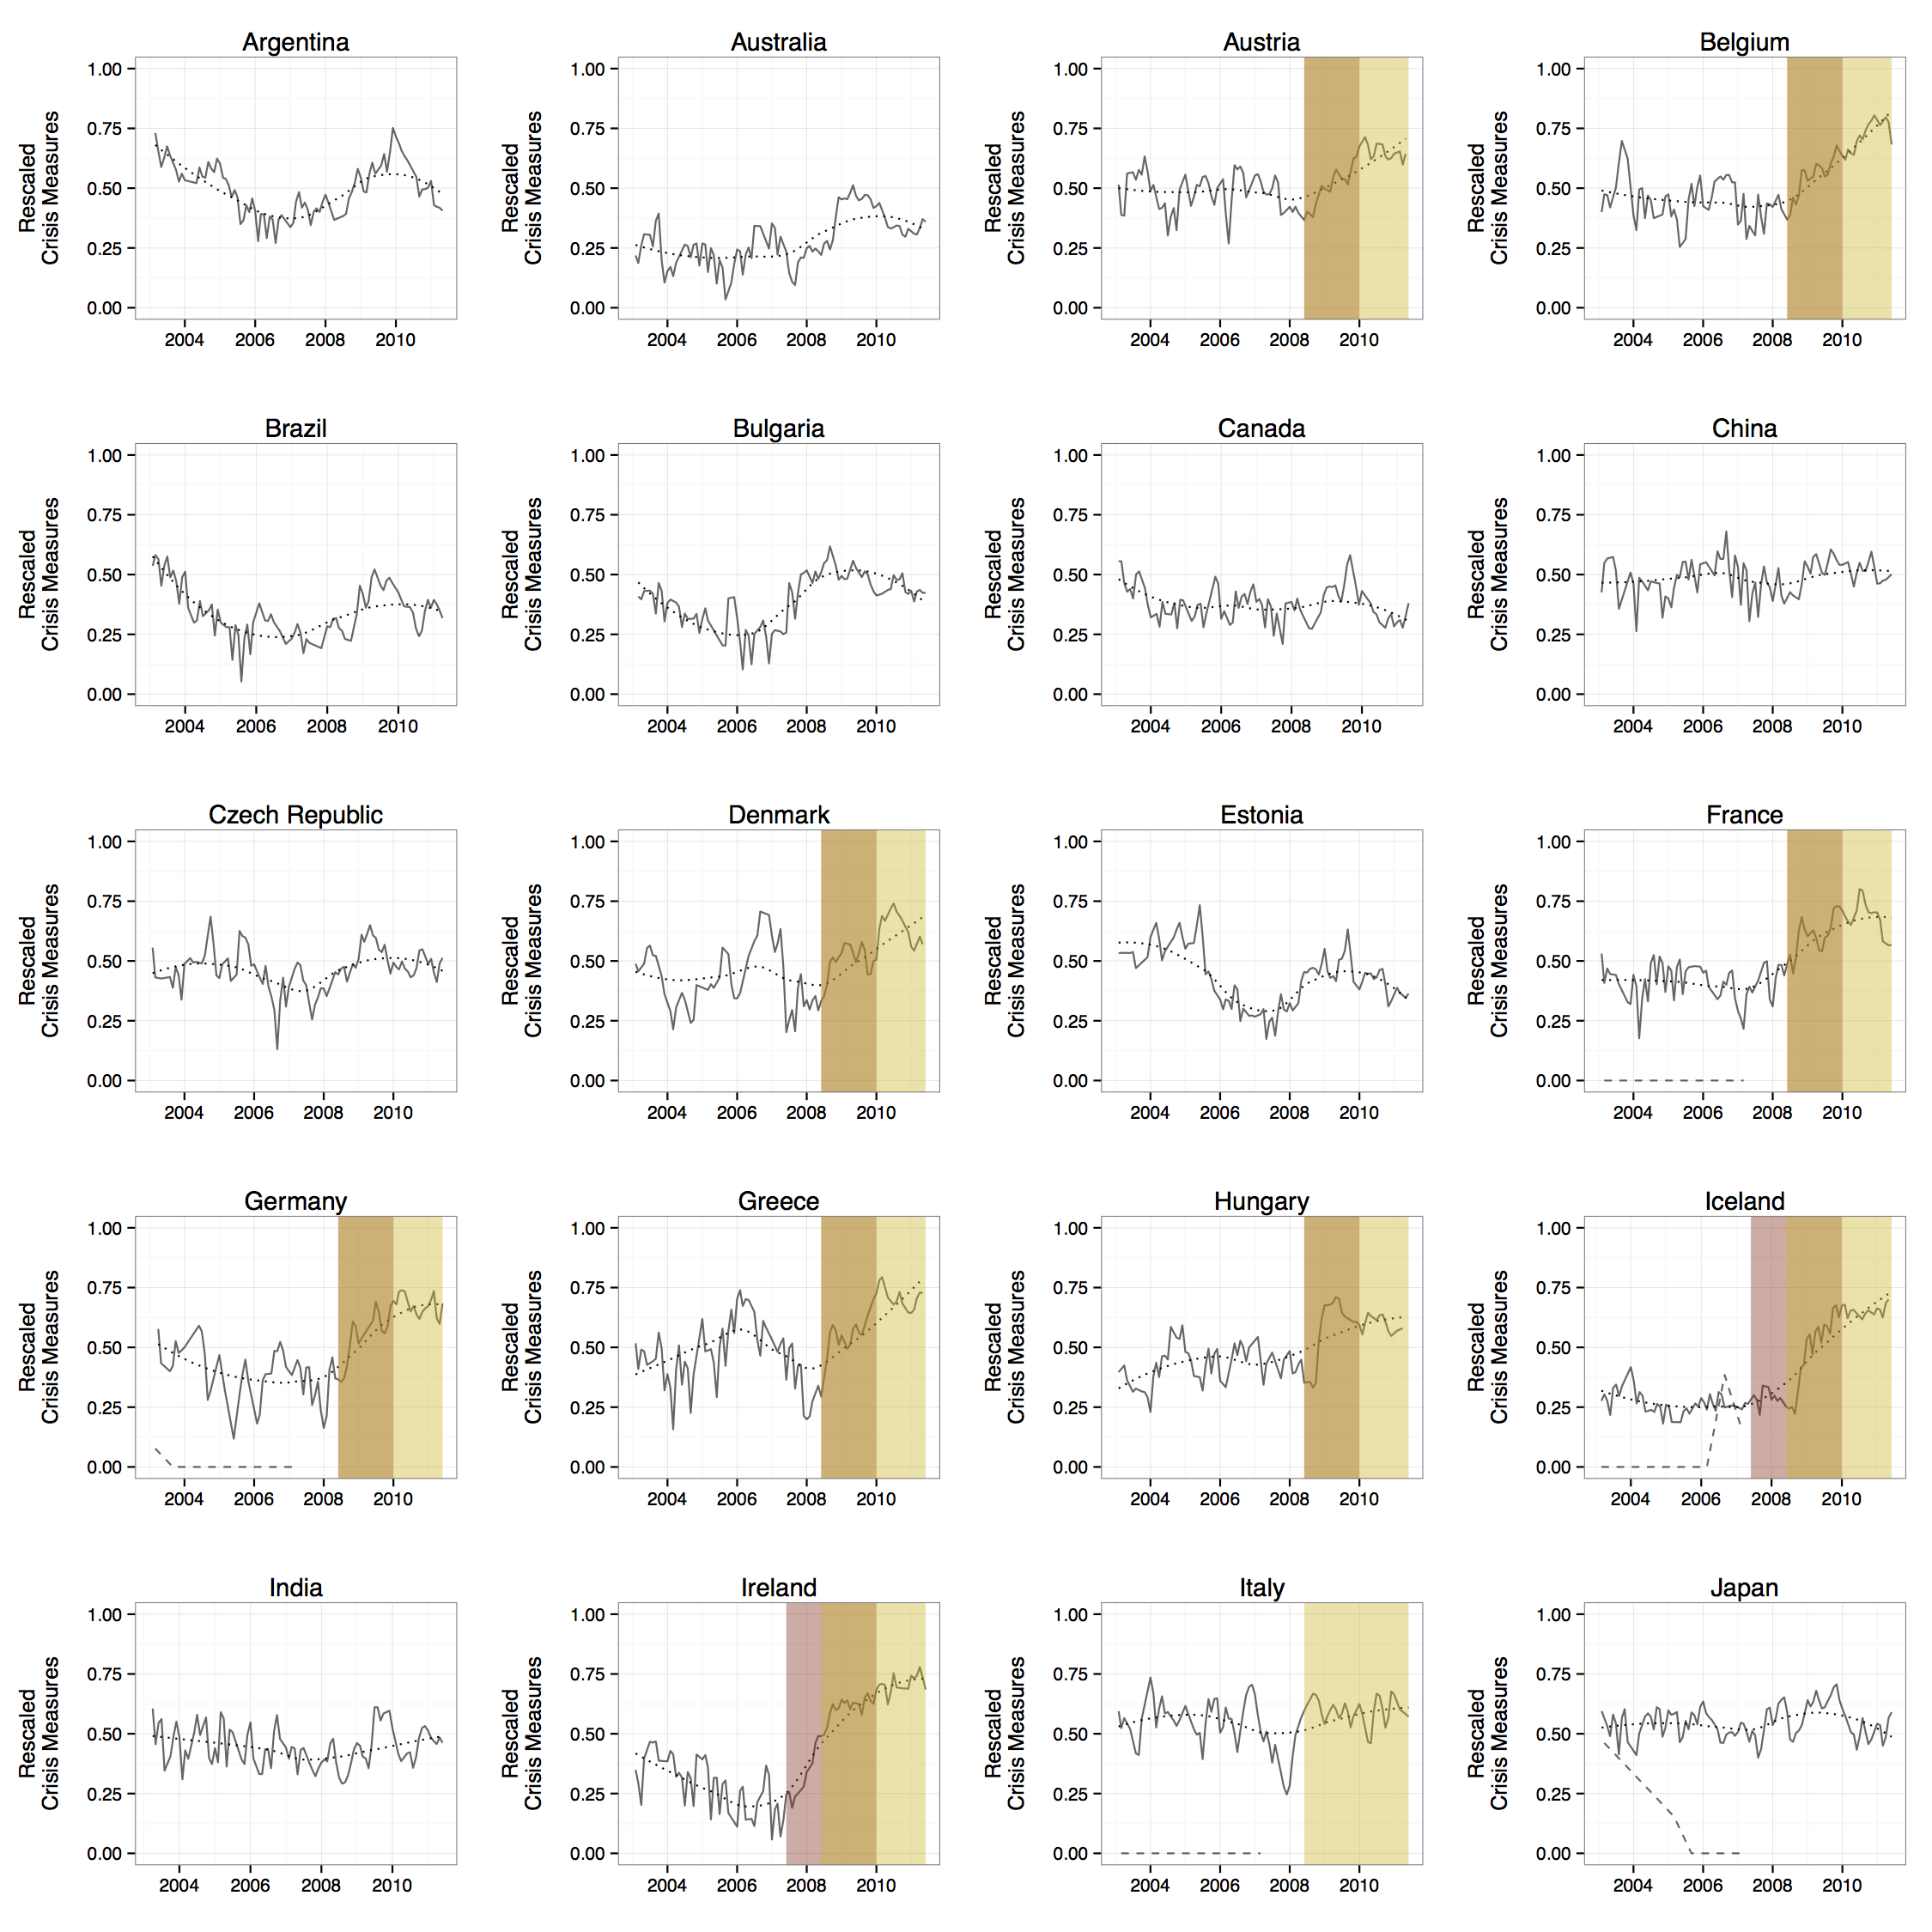
\includegraphics[scale=0.2]{img/perceptions_compare.png}
    \end{center}

    {\tiny{Source: Gandrud and Hallerberg (2016)}}

}

\frame{
    \frametitle{Common output}

    Generally, text analysis results in data that is:

    \begin{itemize}
        \item Nominal: e.g. the main topic of a text.

        \vspace{1cm}

        \item Continuous: e.g. scale (negative to positive, left-right), proportion of a document dedicated to a specific word or words.
    \end{itemize}

}


\section{Human and Machine Coding}

\frame{
    \frametitle{Human vs. Machine coding}

    You can analyse texts either by relying exclusively on human coders or primarily rely on machine-assistance.

    \vspace{1cm}

    Note: you should {\large{never exclusively rely on machine coding}}. At a minimum, you need to check the validity of your machine codes. Do they make sense?

    \vspace{1cm}

    Machine coding has the advantage of being much more {\large{efficient}} for large numbers of texts + more easily {\large{reproducible}}.

}



\end{document}
